\documentclass[11pt,a4paper]{article}

% ------------------------------------------------------------------
% Packages
% ------------------------------------------------------------------
\usepackage[utf8]{inputenc}
\usepackage[T1]{fontenc}
\usepackage{lmodern}
\usepackage[margin=2.5cm]{geometry}
\usepackage{amsmath,amssymb,mathtools}
\usepackage{booktabs}
\usepackage{graphicx}
\usepackage{xcolor}
\usepackage{listings}
\usepackage{caption}
\usepackage{pgfplots}
\usepgfplotslibrary{groupplots}
\pgfplotsset{compat=1.17}
\usetikzlibrary{arrows.meta,positioning,shapes.geometric}
\usepackage[colorlinks=true,linkcolor=blue!60!black,citecolor=blue!60!black,urlcolor=blue!60!black]{hyperref}

% ------------------------------------------------------------------
% Macros
% ------------------------------------------------------------------
\newcommand{\E}{\mathbb{E}}
\newcommand{\Q}{\mathbb{Q}}
\newcommand{\ind}{\mathbf{1}}
\newcommand{\dd}{\mathrm{d}}
\newcommand{\code}[1]{\texttt{#1}}
\newcommand{\Sref}{S_{\mathrm{ref}}}

% Images extracted from the notebooks by make_figures.py ; a framed placeholder is printed while a file is missing.
\newcommand{\figfile}[2]{%
  \IfFileExists{figures/#1}{\includegraphics[width=#2]{figures/#1}}%
  {\fbox{\parbox[c][4cm][c]{#2}{\centering\small missing figure:\\ \texttt{figures/#1}}}}}

\lstset{basicstyle=\ttfamily\footnotesize, keywordstyle=\color{blue!70!black}, commentstyle=\color{gray},
        stringstyle=\color{teal}, frame=single, breaklines=true, language=Python, showstringspaces=false}

\definecolor{athena}{RGB}{31,119,180}
\definecolor{phoenix}{RGB}{214,39,40}
\definecolor{nomemory}{RGB}{255,127,14}
\definecolor{american}{RGB}{44,160,44}

% ------------------------------------------------------------------
\title{Autocallable Notes on the CAC40 under a Calibrated Heston Model:\\
Athena and Phoenix, Fair Coupons, Scenarios and Greeks}
\author{Elias Benguedda}
\date{October 2026}

\begin{document}
\emergencystretch=3em
\maketitle

\begin{abstract}
We price the two main families of single-underlying autocallable notes, the Athena (coupon paid at the call
only) and the Phoenix (periodic conditional coupon, with or without memory), on the CAC40 of 12 February 2025.
The underlying follows a Heston model calibrated to the implied volatility surface (RMSE 0.42 volatility point),
with a drift read from a forward curve bootstrapped from put--call parity. Both products are described by a
single parametrisation covering the observation frequency, snowball or fixed coupons, coupon barrier and memory,
autocall barrier and step-down, non-call period, European, American continuous or American daily capital
protection, airbag and capital guarantee. The notes are priced by Monte Carlo with antithetic variates and a
control variate; the American protection is handled with the Brownian bridge crossing probability as a
conditional expectation. The pricer recovers five closed-form limit cases within one standard error, and an exact identity between the
two families. We report
the fair coupon (price at par) of 35 variants together with their scenario statistics: the base Athena (4 years,
annual observations, autocall at 100\%, European protection at 60\%) pays 9.41\% a year, is called at the first
date with probability 55.7\% and loses capital with probability 9.1\%; the base Phoenix (quarterly, memory, coupon
barrier at 70\%) pays 6.04\% a year. Switching to an American protection adds 1.77 points of coupon to the Athena.
Both notes are short volatility ($-0.55$ and $-0.33$ per vol point on a nominal of 100) and short dividends
($-1.12$ and $-0.32$ per point of carry).
\end{abstract}

\tableofcontents
\newpage

% ==================================================================
\section{Introduction}
% ==================================================================
Autocallable notes are the most widely distributed structured products on equity indices in Europe. The investor
receives coupons well above the risk-free rate, and the note is redeemed early (``called'') as soon as the index is
above a reference level on an observation date. The coupon is financed by a short down-and-in put: if the note
is never called and the index ends below a protection barrier, the investor bears the loss of the index.

Two families cover most of the market:
\begin{itemize}
\item the \textbf{Athena}, whose coupon is paid only when the note is called, usually accumulated over time
(\emph{snowball});
\item the \textbf{Phoenix}, whose coupon is paid at each observation date where the index is above a coupon
barrier, lower than the autocall barrier, usually with a \emph{memory} of the missed coupons.
\end{itemize}
On top of these, issuers combine many features: observation frequency, step-down of the autocall barrier,
non-call period, European or American protection, airbag, capital guarantee. This report prices all of them in a
single framework, on real market data, and measures how each feature moves the fair coupon, the probabilities
of the scenarios and the Greeks.

The model is the Heston model calibrated in \cite{benguedda2026heston} to the CAC40 implied volatility surface,
and the Monte Carlo engine is the one used for barrier options in \cite{benguedda2026barrier}. The scripts and
notebooks are open source; Section~\ref{sec:implementation} describes the code.

% ==================================================================
\section{Products}\label{sec:products}
% ==================================================================

\subsection{Common structure}
A note of nominal $N$ on an index $S$ has an initial fixing $\Sref$ and observation dates
$0 < t_1 < \dots < t_n = T$. The performance at $t_k$ is $P_k = S_{t_k}/\Sref$. All barriers are fractions of
$\Sref$: autocall barriers $B^{\mathrm{call}}_k$, coupon barriers $B^{\mathrm{cpn}}_k$ (Phoenix), protection
barrier $B^{\mathrm{prot}}$. The dates $t_k$ with $t_k \ge t_{\mathrm{nc}}$ are callable, $t_{\mathrm{nc}}$ being the
end of the non-call period; the maturity is always callable. The first callable date where
$P_k \ge B^{\mathrm{call}}_k$ is the call date $\tau$.

\paragraph{Redemption at maturity.} If the note is never called, it is redeemed at $T$ at
\begin{equation}\label{eq:redemption}
R_T = N\left[(1 - \ind_{\mathrm{KI}}) + \ind_{\mathrm{KI}}\,\max\!\Big(\phi,\ \min\big(1,\ P_T/K_{\mathrm{put}}\big)\Big)\right],
\end{equation}
where $\ind_{\mathrm{KI}}$ is the knock-in event of the protection, $K_{\mathrm{put}}$ the strike of the short put
and $\phi$ the capital floor. The knock-in event is
\begin{itemize}
\item \emph{European protection}: $P_T < B^{\mathrm{prot}}$;
\item \emph{American protection}: the index touches $B^{\mathrm{prot}}\Sref$ at any time before maturity,
continuously or on daily closes.
\end{itemize}
The standard note has $K_{\mathrm{put}} = 1$ and $\phi = 0$: below the barrier, the investor receives
$N P_T$ and the redemption jumps from $N$ to $N B^{\mathrm{prot}}$ at the barrier. The \emph{airbag} note has
$K_{\mathrm{put}} = B^{\mathrm{prot}}$: the redemption is continuous at the barrier and equal to
$N P_T / B^{\mathrm{prot}}$ below it. A \emph{capital guarantee} sets $\phi > 0$. Figure~\ref{fig:redemption}
draws the three profiles.

\begin{figure}[h]
\centering
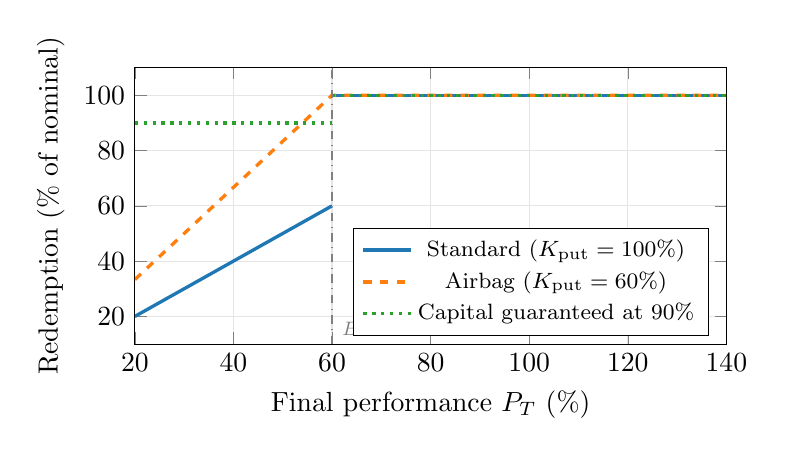
\begin{tikzpicture}
\begin{axis}[width=0.75\textwidth, height=0.42\textwidth, xmin=20, xmax=140, ymin=10, ymax=110,
             xlabel={Final performance $P_T$ (\%)}, ylabel={Redemption (\% of nominal)},
             grid=major, grid style={gray!20}, legend pos=south east, legend style={font=\footnotesize}]
\addplot[athena, very thick] coordinates {(20,20) (60,60)};
\addplot[athena, very thick, forget plot] coordinates {(60,100) (140,100)};
\addplot[nomemory, very thick, dashed] coordinates {(20,33.33) (60,100) (140,100)};
\addplot[american, very thick, dotted] coordinates {(20,90) (60,90)};
\addplot[american, very thick, dotted, forget plot] coordinates {(60,100) (140,100)};
\draw[gray, dashdotted] (axis cs:60,10) -- (axis cs:60,110) node[pos=0.06, right, font=\scriptsize] {$B^{\mathrm{prot}} = 60\%$};
\legend{Standard ($K_{\mathrm{put}} = 100\%$), Airbag ($K_{\mathrm{put}} = 60\%$), Capital guaranteed at 90\%}
\end{axis}
\end{tikzpicture}
\caption{Redemption at maturity of a note that was never called, European protection at 60\%.}
\label{fig:redemption}
\end{figure}

\subsection{Athena}
The Athena pays a coupon only with the redemption at the call date. If $\tau = t_k$, the investor receives
\begin{equation}
N(1 + c_k), \qquad c_k = \begin{cases} c\, t_k & \text{snowball (the coupons accumulate)}, \\ c\,(t_k - t_{k-1}) & \text{fixed coupon}, \end{cases}
\end{equation}
with $c$ the coupon rate per annum. If the note is not called, no coupon is paid and the redemption is
\eqref{eq:redemption}. A call at maturity ($P_T \ge B^{\mathrm{call}}_n$) pays the last coupon.

\subsection{Phoenix}
The Phoenix pays at each observation date $t_k \le \tau$ (and $t_k \le T$) the coupon
\begin{equation}
N\, c\,(t_k - t_{k-1})\, \ind_{\{P_k \ge B^{\mathrm{cpn}}_k\}}
\end{equation}
and, with memory, the coupons of all the previous dates since the last payment. When the note is called, it is
redeemed at $N$. With $B^{\mathrm{cpn}}_k = 0$, the coupon is unconditional; with
$B^{\mathrm{cpn}}_k = B^{\mathrm{call}}_k$ and memory, a coupon is paid only at the call date and its amount is
$c\, t_k$: the Phoenix is then exactly a snowball Athena (Table~\ref{tab:validation} checks it numerically).
Figure~\ref{fig:decision} summarises the decisions taken at an observation date.

\begin{figure}[h]
\centering
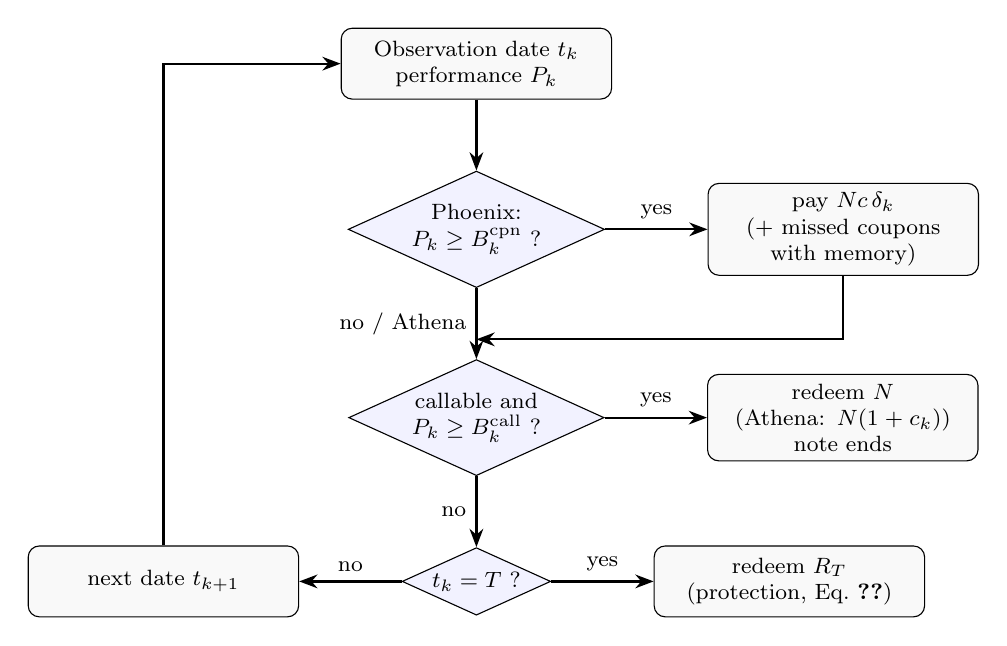
\begin{tikzpicture}[node distance=0.9cm and 1.3cm, font=\footnotesize,
    box/.style={draw, rounded corners, align=center, minimum height=0.9cm, text width=3.2cm, fill=gray!5},
    test/.style={draw, diamond, aspect=2.2, align=center, inner sep=1pt, fill=blue!5},
    arrow/.style={-{Stealth}, thick}]
\node[box] (obs) {Observation date $t_k$\\ performance $P_k$};
\node[test, below=of obs] (cpn) {Phoenix:\\ $P_k \ge B^{\mathrm{cpn}}_k$ ?};
\node[box, right=of cpn] (pay) {pay $N c\,\delta_k$\\ (+ missed coupons\\ with memory)};
\node[test, below=of cpn] (call) {callable and\\ $P_k \ge B^{\mathrm{call}}_k$ ?};
\node[box, right=of call] (red) {redeem $N$\\ (Athena: $N(1 + c_k)$)\\ note ends};
\node[test, below=of call] (last) {$t_k = T$ ?};
\node[box, right=of last] (mat) {redeem $R_T$\\ (protection, Eq.~\ref{eq:redemption})};
\node[box, left=of last] (next) {next date $t_{k+1}$};
\draw[arrow] (obs) -- (cpn);
\draw[arrow] (cpn) -- node[above] {yes} (pay);
\draw[arrow] (cpn) -- node[left] {no / Athena} (call);
\draw[arrow] (pay) |- ([yshift=0.25cm]call.north);
\draw[arrow] (call) -- node[above] {yes} (red);
\draw[arrow] (call) -- node[left] {no} (last);
\draw[arrow] (last) -- node[above] {yes} (mat);
\draw[arrow] (last) -- node[above] {no} (next);
\draw[arrow] (next) |- (obs);
\end{tikzpicture}
\caption{Cash flows of an autocallable note at an observation date.}
\label{fig:decision}
\end{figure}

\subsection{Parametrisation}
Table~\ref{tab:parameters} lists the parameters of the classes \code{Athena} and \code{Phoenix}; every variant of
Sections~\ref{sec:athena} and~\ref{sec:phoenix} is one of these parameters changed.

\begin{table}[h]
\centering
\resizebox{\textwidth}{!}{%
\begin{tabular}{@{}lll@{}}
\toprule
\textbf{Feature} & \textbf{Parameter} & \textbf{Values} \\
\midrule
Maturity, initial fixing, nominal & \code{maturity}, \code{initial\_fixing}, \code{nominal} & years, index level, 100 \\
Observation dates & \code{frequency} or \code{observation\_dates} & monthly to annual, or any list ending at $T$ \\
Coupon rate & \code{coupon\_rate} & per annum, fraction of the nominal \\
Athena coupon & \code{coupon\_type} & \code{snowball}, \code{fixed} \\
Phoenix coupon & \code{coupon\_barrier}, \code{memory} & fraction of $\Sref$ (scalar or one per date), True / False \\
Autocall barrier & \code{autocall\_barrier}, \code{step\_down} & fraction of $\Sref$, decrease per observation \\
Non-call period & \code{first\_call\_date} & years \\
Capital protection & \code{protection\_barrier}, \code{protection\_type} & fraction of $\Sref$; \code{european}, \code{american}, \code{american\_discrete} \\
Airbag, guarantee & \code{put\_strike}, \code{floor} & fraction of $\Sref$, fraction of the nominal \\
\bottomrule
\end{tabular}}
\caption{Parameters of the autocallable notes (\code{Produits/products.py}).}
\label{tab:parameters}
\end{table}

% ==================================================================
\section{Market Data and Model}\label{sec:model}
% ==================================================================
The data are the CAC40 option chain of 12 February 2025 (spot $S_0 = 8042.19$, 142 quotes on 13 expiries from
9 days to 4.86 years) and the EURIBOR 6M zero-coupon curve. The forward curve $F(0,t)$ is bootstrapped from
put--call parity with a piecewise constant borrow-plus-dividend yield $q(t)$ \cite{benguedda2026heston}; its
integral reaches 0.136 at 4.86 years, so dividends lower the 4-year forward by about 11\% with respect to a zero
carry. Under $\Q$,
\begin{equation}
\frac{\dd S_t}{S_t} = \partial_t \ln F(0,t)\,\dd t + \sqrt{v_t}\,\dd W^S_t, \qquad
\dd v_t = \kappa(\theta - v_t)\,\dd t + \xi \sqrt{v_t}\,\dd W^v_t, \qquad \dd\langle W^S, W^v\rangle_t = \rho\,\dd t,
\end{equation}
with the parameters of Table~\ref{tab:heston}. The notes are struck at the money: $\Sref = S_0 = 8042.19$, and
$\Sref$ stays fixed when the Greeks bump the market. All the dates of the 4-year notes lie before the last listed
expiry (4.86 years).

\begin{table}[h]
\centering
\begin{tabular}{@{}cccccc@{}}
\toprule
$v_0$ & $\theta$ & $\kappa$ & $\xi$ & $\rho$ & IV RMSE \\
\midrule
0.0197 & 0.0438 & 1.308 & 0.482 & $-0.605$ & 0.421 vol pts \\
\bottomrule
\end{tabular}
\caption{Heston parameters calibrated on the CAC40 surface of 12 February 2025 \cite{benguedda2026heston}.}
\label{tab:heston}
\end{table}

% ==================================================================
\section{Pricing Method}\label{sec:method}
% ==================================================================

\subsection{Simulation}
The paths of $(S, v)$ are simulated with an Euler full truncation scheme on a weekly grid (52 steps a year,
208 steps for 4 years), the drift over each step being $\ln(F(0,t_{i+1})/F(0,t_i))$, so that
$\E[S_t] = F(0,t)$ at every date. $N = 50{,}000$ paths with antithetic variates are used (seed 42); prices and
standard errors are computed on the 25{,}000 independent pair averages. The observation dates are rounded to the
grid; with weekly steps, every monthly, quarterly, semi-annual and annual date falls within half a week of its
contractual date.

\subsection{Cash flows and protection}
For each path, the note is followed through its observation dates (Figure~\ref{fig:decision}), each cash flow
being discounted with $D(0,t_k) = e^{-r(t_k) t_k}$. The knock-in indicator of \eqref{eq:redemption} is
\begin{itemize}
\item \emph{European}: $\ind_{\{P_T < B^{\mathrm{prot}}\}}$;
\item \emph{American continuous}: replaced by its conditional probability given the simulated path,
$1 - \prod_i (1 - p_i)$, where
$p_i = \exp\!\big(-2 \ln(S_{t_i}/H) \ln(S_{t_{i+1}}/H) / (v_{t_i}\Delta t)\big)$ is the probability that the
Brownian bridge of $\ln S$ touches $H = B^{\mathrm{prot}}\Sref$ between two grid dates \cite{beaglehole1997};
\item \emph{American daily}: the barrier is checked on a daily grid (252 steps a year).
\end{itemize}

\subsection{Variance reduction}
Besides antithetic variates, the discounted European put struck at $B^{\mathrm{prot}}\Sref$, whose Heston price
is known semi-analytically (Lewis formula), is used as a control variate with an optimal coefficient estimated on
the paths.

\subsection{Fair coupon and scenario statistics}
On a fixed set of paths, the call dates do not depend on the coupon, and every cash flow is affine in the coupon
rate $c$: the price is $V(c) = V(0) + c\,(V(1) - V(0))$, and the coupon that prices the note at par is
\begin{equation}
c^\star = \frac{N - V(0)}{V(1) - V(0)},
\end{equation}
obtained with two valuations. It excludes the issuer margin and funding spread. The same paths give the
probability of a call at each date, the probability to reach maturity, the probability of a capital loss
($\ind_{\mathrm{KI}} = 1$ and $P_T < K_{\mathrm{put}}$), the expected loss at maturity, the expected life
$\E[\min(\tau, T)]$ and the expected number of coupons.

\subsection{Greeks}
The Greeks are central finite differences with common random numbers \cite{glasserman2004}, on a nominal of 100:
Delta and Gamma (spot $\pm 1\%$, carry kept), Vega and Volga ($\sqrt{v_0}$ and $\sqrt{\theta}$ shifted by
$\pm 1$ vol point), Vanna, Rho ($\pm 10$bp on the zero curve, per $+1\%$), Dividend ($\pm 10$bp on $q(t)$, per
$+1\%$) and Theta (dates moved by one day). Delta is given per index point: multiply by $S_0/100 = 80.4$ for the
value change of a 1\% move. Each Greek is reported with its Monte Carlo standard error.

\subsection{Validation}
Five limit cases have a closed form or an exact counterpart (Table~\ref{tab:validation}). In a flat Black--Scholes
market ($S_0 = \Sref = 100$, $r = 3\%$, $q = 1\%$, $\sigma = 20\%$, $T = 2$, $N = 100$, Heston with $v_0 = \theta = \sigma^2$
and $\xi = 10^{-4}$, $10^5$ paths):
\begin{itemize}
\item a note never called (autocall barrier out of reach) with a European protection at $B = 60$ is worth
$N D(T) - \frac{N}{\Sref}\left[\mathrm{Put}(B) + (\Sref - B)\,\mathrm{DigitalPut}(B)\right]$;
\item with an American protection, $N D(T) - \frac{N}{\Sref}\,\mathrm{PDI}(K = \Sref, H = B)$ (Reiner--Rubinstein);
\item a note called for sure at $t_1$ is worth $N(1 + c\, t_1) D(t_1)$;
\item a Phoenix never called with unconditional quarterly coupons is worth the sum of its discounted coupons plus
the first case.
\end{itemize}
On the CAC40, the Phoenix with memory and $B^{\mathrm{cpn}} = B^{\mathrm{call}}$ must have exactly the price of the
snowball Athena with the same dates.

\begin{table}[h]
\centering
\resizebox{\textwidth}{!}{%
\begin{tabular}{@{}lrrrr@{}}
\toprule
\textbf{Case} & \textbf{Reference} & \textbf{Monte Carlo} & \textbf{Std error} & \textbf{Error / std error} \\
\midrule
Athena never called, European protection (flat) & 92.6369 & 92.6480 & 0.0141 & 0.79 \\
Athena never called, American protection (flat) & 91.5500 & 91.5483 & 0.0220 & $-0.07$ \\
Athena called for sure at $t_1 = 0.5$, $c = 8\%$ (flat) & 102.4516 & 102.4516 & 0 & exact \\
Phoenix never called, unconditional 6\% coupon (flat) & 104.2404 & 104.2515 & 0.0141 & 0.79 \\
Phoenix called for sure at $t_1 = 0.25$, $c = 6\%$ (flat) & 100.742 & 100.742 & 0 & exact \\
Phoenix with memory, $B^{\mathrm{cpn}} = B^{\mathrm{call}}$ vs snowball Athena (CAC40) & 98.7669 & 98.7669 & 0.0585 & identical paths \\
\bottomrule
\end{tabular}}
\caption{Validation of the pricer.}
\label{tab:validation}
\end{table}

% ==================================================================
\section{Athena}\label{sec:athena}
% ==================================================================

\subsection{Base case}
The base Athena has a maturity of 4 years, annual observations, a snowball coupon of 8\% a year, an autocall
barrier at 100\% and a European protection at 60\%. Its price is $98.596 \pm 0.128$ (95\%) for a nominal of 100,
and its fair coupon is $9.41\%$ a year. Table~\ref{tab:athena_base} gives the scenario statistics and
Figure~\ref{fig:call_probabilities} the call probabilities: more than half of the notes are called after one year,
a quarter reaches maturity, and 9.1\% lose capital, with an expected loss of 5.27\% of the nominal (58\% of the
nominal given a loss).

\begin{table}[h]
\centering
\begin{tabular}{@{}lr@{\qquad}lr@{}}
\toprule
Call at 1 year & 55.69\% & Probability to reach maturity & 25.70\% \\
Call at 2 years & 10.83\% & Probability of a capital loss & 9.06\% \\
Call at 3 years & 4.81\% & Expected loss at maturity & 5.27\% \\
Call at 4 years & 2.96\% & Expected life & 2.06 years \\
\bottomrule
\end{tabular}
\caption{Base Athena: scenario statistics on 50{,}000 paths.}
\label{tab:athena_base}
\end{table}

\begin{figure}[h]
\centering
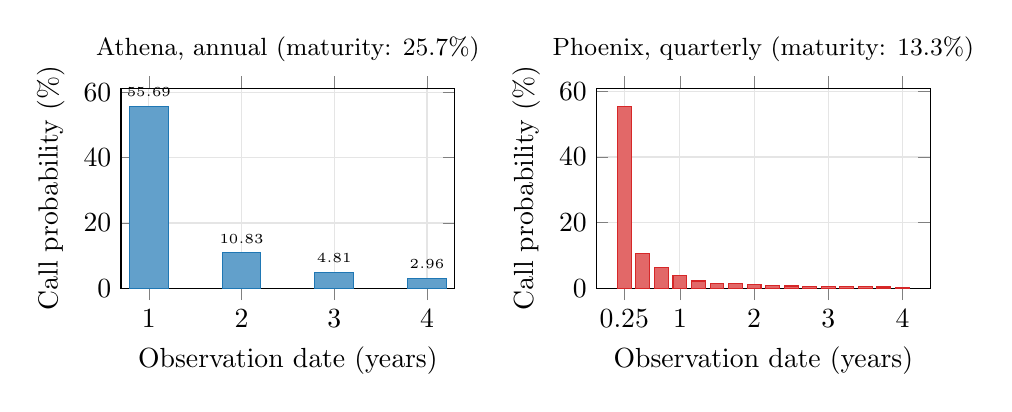
\begin{tikzpicture}
\begin{groupplot}[group style={group size=2 by 1, horizontal sep=1.8cm},
  width=0.48\textwidth, height=0.34\textwidth, ymin=0, ylabel={Call probability (\%)},
  grid=major, grid style={gray!20}, title style={font=\small}]
\nextgroupplot[ybar, bar width=14pt, xlabel={Observation date (years)}, xtick={1,2,3,4},
               title={Athena, annual (maturity: 25.7\%)}, nodes near coords, every node near coord/.append style={font=\tiny}]
\addplot[fill=athena!70, draw=athena] coordinates {(1,55.69) (2,10.83) (3,4.81) (4,2.96)};
\nextgroupplot[ybar, bar width=5pt, xlabel={Observation date (years)}, xtick={0.25,1,2,3,4},
               title={Phoenix, quarterly (maturity: 13.3\%)}]
\addplot[fill=phoenix!70, draw=phoenix] coordinates {(0.25,55.43) (0.5,10.63) (0.75,6.24) (1,3.86) (1.25,2.21) (1.5,1.57)
  (1.75,1.41) (2,1.13) (2.25,0.82) (2.5,0.69) (2.75,0.59) (3,0.51) (3.25,0.46) (3.5,0.47) (3.75,0.39) (4,0.30)};
\end{groupplot}
\end{tikzpicture}
\caption{Probability of being called at each observation date (autocall barrier at 100\%).}
\label{fig:call_probabilities}
\end{figure}

\begin{figure}[h]
\centering
\figfile{athena_scenarios.png}{0.9\textwidth}
\caption{Base Athena: simulated paths of the performance, grouped by outcome.}
\label{fig:athena_scenarios}
\end{figure}

\subsection{All the forms of the Athena}
Table~\ref{tab:athena_variants} changes one feature of the base case at a time. All prices are computed at
the same coupon of 8\% (standard errors between 0.03 and 0.08); the fair coupon is the comparable quantity.

\begin{table}[h]
\centering
\resizebox{\textwidth}{!}{%
\begin{tabular}{@{}lrrrrrrr@{}}
\toprule
\textbf{Variant} & \textbf{Price at 8\%} & \textbf{Fair coupon} & \textbf{P(call $t_1$)} & \textbf{P(maturity)} & \textbf{P(loss)} & \textbf{E[loss]} & \textbf{E[life]} \\
 & & \textbf{(\% p.a.)} & \textbf{(\%)} & \textbf{(\%)} & \textbf{(\%)} & \textbf{(\%)} & \textbf{(y)} \\
\midrule
Base (annual, snowball, AC 100\%, EU 60\%) & 98.60 & 9.41 & 55.69 & 25.70 & 9.06 & 5.27 & 2.06 \\
Semi-annual observations & 98.64 & 9.93 & 53.30 & 18.61 & 6.97 & 4.08 & 1.48 \\
Quarterly observations & 98.77 & 10.54 & 55.43 & 13.29 & 5.22 & 3.05 & 1.03 \\
Monthly observations & 99.16 & 11.11 & 56.21 & 7.77 & 3.13 & 1.83 & 0.59 \\
Fixed coupon (no snowball) & 96.40 & 13.00 & 55.69 & 25.70 & 9.06 & 5.27 & 2.06 \\
Autocall barrier 90\% & 100.95 & 7.03 & 77.37 & 13.24 & 6.41 & 3.77 & 1.54 \\
Autocall barrier 110\% & 95.40 & 12.71 & 25.07 & 45.60 & 11.77 & 6.77 & 2.85 \\
Step-down 5\% per year & 100.65 & 7.46 & 55.69 & 17.56 & 8.57 & 5.01 & 1.95 \\
Quarterly, non-call 1 year & 99.09 & 8.94 & 0.00 & 22.06 & 8.42 & 4.92 & 1.89 \\
Protection 50\% & 99.90 & 8.10 & 55.69 & 25.70 & 5.91 & 3.86 & 2.06 \\
Protection 70\% & 97.33 & 10.68 & 55.69 & 25.70 & 12.96 & 6.63 & 2.06 \\
American protection (continuous) & 96.83 & 11.18 & 55.69 & 25.70 & 16.43 & 7.20 & 2.06 \\
American protection (daily) & 96.95 & 11.05 & 55.53 & 25.67 & 16.07 & 7.18 & 2.07 \\
Airbag & 100.89 & 7.10 & 55.69 & 25.70 & 9.06 & 2.75 & 2.06 \\
Capital guaranteed 90\% & 102.56 & 5.42 & 55.69 & 25.70 & 9.06 & 0.91 & 2.06 \\
Capital guaranteed 100\% & 103.39 & 4.59 & 55.69 & 25.70 & 0.00 & 0.00 & 2.06 \\
\bottomrule
\end{tabular}}
\caption{Athena variants on the CAC40 (Heston, 50{,}000 paths). E[loss] in \% of the nominal.}
\label{tab:athena_variants}
\end{table}

\paragraph{Reading the table.} The investor is short a down-and-in put whose premium is paid back through the
coupons; the fair coupon per annum is roughly this premium divided by the expected life of the note.
\begin{itemize}
\item \emph{Observation frequency.} More frequent observations call the note earlier (expected life from 2.06 to
0.59 years) and reduce the probability of a loss (from 9.06\% to 3.13\%), but the put premium is spread over a much
shorter life: the fair coupon rises from 9.41\% to 11.11\%.
\item \emph{Snowball vs fixed coupon.} A fixed coupon pays $c$ once whatever the call date, instead of $c\,t_k$:
the fair coupon is 13.00\% instead of 9.41\%.
\item \emph{Autocall barrier.} A barrier at 90\% calls 77\% of the notes after one year and lowers the fair coupon
to 7.03\%; at 110\%, 46\% of the notes reach maturity and the fair coupon is 12.71\%. A step-down of 5\% a year
lowers it to 7.46\%.
\item \emph{Protection.} Each 5 points of protection barrier move the fair coupon by 0.4 to 0.7 point
(Figure~\ref{fig:fair_coupon}). The American protection raises the probability of a loss from 9.06\% to 16.43\% and
the fair coupon by 1.77 points; a daily monitoring lowers the fair coupon by 0.13 point with respect to a continuous
monitoring.
\item \emph{Airbag and guarantee.} The airbag halves the expected loss (2.75\% instead of 5.27\%) for a coupon of
7.10\%; a 100\% capital guarantee leaves a coupon of 4.59\%, the value of the call-at-par feature on top of a
zero-coupon bond.
\end{itemize}

\begin{figure}[h]
\centering
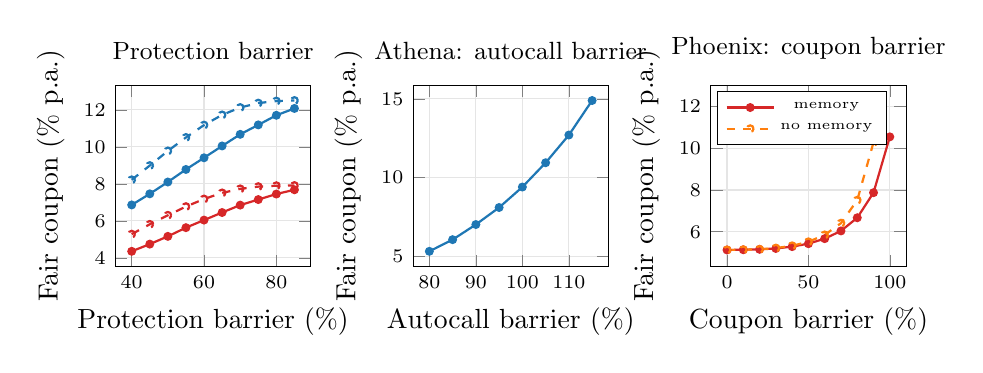
\begin{tikzpicture}
\begin{groupplot}[group style={group size=3 by 1, horizontal sep=1.3cm},
  width=0.335\textwidth, height=0.32\textwidth, ylabel={Fair coupon (\% p.a.)}, grid=major, grid style={gray!20},
  title style={font=\small}, legend style={font=\tiny, at={(0.03,0.97)}, anchor=north west}, ticklabel style={font=\scriptsize}]
\nextgroupplot[xlabel={Protection barrier (\%)}, title={Protection barrier},
               legend columns=4, legend to name=fairlegend, legend style={font=\footnotesize, /tikz/every even column/.append style={column sep=0.4cm}}]
\addplot[athena, thick, mark=*, mark size=1.2pt] coordinates {(40,6.86) (45,7.46) (50,8.10) (55,8.78) (60,9.41) (65,10.05) (70,10.68) (75,11.19) (80,11.71) (85,12.08)};
\addplot[athena, thick, dashed, mark=o, mark size=1.2pt] coordinates {(40,8.22) (45,8.99) (50,9.78) (55,10.51) (60,11.18) (65,11.73) (70,12.13) (75,12.37) (80,12.48) (85,12.51)};
\addplot[phoenix, thick, mark=*, mark size=1.2pt] coordinates {(40,4.35) (45,4.74) (50,5.16) (55,5.63) (60,6.04) (65,6.45) (70,6.85) (75,7.15) (80,7.45) (85,7.68)};
\addplot[phoenix, thick, dashed, mark=o, mark size=1.2pt] coordinates {(40,5.28) (45,5.81) (50,6.30) (55,6.77) (60,7.18) (65,7.51) (70,7.73) (75,7.85) (80,7.90) (85,7.91)};
\legend{Athena EU, Athena AM, Phoenix EU, Phoenix AM}
\nextgroupplot[xlabel={Autocall barrier (\%)}, title={Athena: autocall barrier}]
\addplot[athena, thick, mark=*, mark size=1.2pt] coordinates {(80,5.33) (85,6.07) (90,7.03) (95,8.11) (100,9.41) (105,10.95) (110,12.71) (115,14.90)};
\nextgroupplot[xlabel={Coupon barrier (\%)}, title={Phoenix: coupon barrier}, ymax=13]
\addplot[phoenix, thick, mark=*, mark size=1.2pt] coordinates {(0,5.13) (10,5.14) (20,5.16) (30,5.20) (40,5.29) (50,5.43) (60,5.67) (70,6.04) (80,6.67) (90,7.87) (100,10.54)};
\addplot[nomemory, thick, dashed, mark=o, mark size=1.2pt] coordinates {(0,5.13) (10,5.14) (20,5.16) (30,5.22) (40,5.33) (50,5.52) (60,5.85) (70,6.41) (80,7.51) (90,10.28)};
\legend{memory, no memory}
\end{groupplot}
\end{tikzpicture}\\[1mm]
\pgfplotslegendfromname{fairlegend}
\caption{Fair coupons as functions of the barriers (other features of the base cases unchanged; EU / AM: European /
American continuous protection). The Phoenix without memory reaches 23.94\% at a coupon barrier of 100\% (off scale).}
\label{fig:fair_coupon}
\end{figure}

\subsection{Greeks}
Table~\ref{tab:athena_greeks} gives the Greeks of five Athena variants. Gamma and Volga are not significant at
this number of paths (base case: Gamma $-3.0 \times 10^{-6} \pm 5.4 \times 10^{-6}$, Volga $-0.042 \pm 0.037$);
the other Greeks have relative standard errors between 3\% and 45\% (base case: Delta $0.00506 \pm 0.00019$, Vega
$-0.549 \pm 0.016$, Rho $-0.77 \pm 0.07$, Dividend $-1.12 \pm 0.07$, Theta $0.0050 \pm 0.0016$).

\begin{table}[h]
\centering
\resizebox{\textwidth}{!}{%
\begin{tabular}{@{}lrrrrrrrr@{}}
\toprule
\textbf{Athena} & \textbf{Price} & \textbf{Delta} & \textbf{Delta 1\%} & \textbf{Vega} & \textbf{Vanna} & \textbf{Rho} & \textbf{Dividend} & \textbf{Theta} \\
 & & (per point) & (per 1\% move) & (per vol pt) & ($\times 10^{4}$) & (per 1\%) & (per 1\%) & (per day) \\
\midrule
Base & 98.60 & 0.00506 & 0.407 & $-0.549$ & 2.51 & $-0.770$ & $-1.115$ & 0.0050 \\
American protection & 96.83 & 0.00644 & 0.518 & $-0.657$ & 1.97 & $-0.546$ & $-1.269$ & 0.0050 \\
Step-down 5\% & 100.65 & 0.00321 & 0.258 & $-0.637$ & 6.36 & $-0.900$ & $-0.935$ & 0.0079 \\
Airbag & 100.89 & 0.00343 & 0.276 & $-0.354$ & 1.28 & $-1.161$ & $-0.815$ & 0.0037 \\
Guaranteed 90\% & 102.56 & 0.00241 & 0.193 & $-0.139$ & 0.44 & $-1.436$ & $-0.608$ & 0.0023 \\
\bottomrule
\end{tabular}}
\caption{Greeks of Athena variants (nominal 100, coupon 8\%).}
\label{tab:athena_greeks}
\end{table}

The note is long the index (a 1\% rise is worth 0.41 on 100) and short volatility: one vol point costs 0.55, the
short put dominating the long digital-like call features. It is also short dividends: one point of carry lowers
every forward and costs 1.12, twice the vega. It loses with higher rates (discounting of the coupons and of the
nominal) and earns about 0.005 a day (1.8 a year) as the put decays. The capital guarantee reduces every risk but
the rate risk, since the guaranteed redemption behaves as a zero-coupon bond. Figure~\ref{fig:athena_greeks}
displays the table with 95\% confidence intervals and Figure~\ref{fig:athena_profiles} the Greeks as functions of
the spot, the initial fixing staying at 8042: the Delta increases as the spot falls towards the protection barrier
(4825), and peaks just above it with an American protection.

\begin{figure}[h]
\centering
\figfile{athena_greeks.png}{\textwidth}
\caption{Greeks of the Athena variants with 95\% confidence intervals.}
\label{fig:athena_greeks}
\end{figure}

\begin{figure}[h]
\centering
\figfile{athena_profiles.png}{\textwidth}
\caption{Athena: price and Greeks as functions of the spot (30{,}000 paths, spot step 400).}
\label{fig:athena_profiles}
\end{figure}

\paragraph{Sensitivities to the Heston parameters.} Per unit of parameter, the base Athena has
$\partial V/\partial v_0 = -69.9$, $\partial V/\partial \theta = -69.4$, $\partial V/\partial \kappa = -0.81$,
$\partial V/\partial \xi = 3.94$ and $\partial V/\partial \rho = -1.03$. The note loses with the variance level
(short put) and gains with the vol-of-vol $\xi$.

% ==================================================================
\section{Phoenix}\label{sec:phoenix}
% ==================================================================

\subsection{Base case}
The base Phoenix has a maturity of 4 years, quarterly observations, a coupon of 6\% a year (1.5\% a quarter)
with memory and a coupon barrier at 70\%, an autocall barrier at 100\% and a European protection at 60\%. Its price
is $99.963 \pm 0.099$ (95\%) and its fair coupon $6.04\%$ a year. 55.4\% of the notes are called after one
quarter (Figure~\ref{fig:call_probabilities}), the expected life is 1.03 years, 3.28 coupons are paid on
average, 13.3\% of the notes reach maturity and 5.2\% lose capital, with an expected loss of 3.05\%.

\begin{figure}[h]
\centering
\figfile{phoenix_scenarios.png}{0.9\textwidth}
\caption{Base Phoenix: simulated paths of the performance, grouped by outcome.}
\label{fig:phoenix_scenarios}
\end{figure}

\subsection{All the forms of the Phoenix}

\begin{table}[h]
\centering
\resizebox{\textwidth}{!}{%
\begin{tabular}{@{}lrrrrrrr@{}}
\toprule
\textbf{Variant} & \textbf{Price at 6\%} & \textbf{Fair coupon} & \textbf{P(maturity)} & \textbf{P(loss)} & \textbf{E[loss]} & \textbf{E[life]} & \textbf{E[coupons]} \\
 & & \textbf{(\% p.a.)} & \textbf{(\%)} & \textbf{(\%)} & \textbf{(\%)} & \textbf{(y)} & \\
\midrule
Base (quarterly, memory, CB 70\%) & 99.96 & 6.04 & 13.29 & 5.22 & 3.05 & 1.03 & 3.28 \\
No memory & 99.67 & 6.41 & 13.29 & 5.22 & 3.05 & 1.03 & 3.28 \\
Coupon barrier 50\% & 100.54 & 5.43 & 13.29 & 5.22 & 3.05 & 1.03 & 3.83 \\
Coupon barrier 60\% & 100.30 & 5.67 & 13.29 & 5.22 & 3.05 & 1.03 & 3.61 \\
Coupon barrier 80\% & 99.49 & 6.67 & 13.29 & 5.22 & 3.05 & 1.03 & 2.80 \\
Coupon barrier = autocall barrier (= snowball Athena) & 97.80 & 10.54 & 13.29 & 5.22 & 3.05 & 1.03 & 0.87 \\
Unconditional coupon (CB 0\%) & 100.87 & 5.13 & 13.29 & 5.22 & 3.05 & 1.03 & 4.13 \\
Monthly observations & 99.91 & 6.19 & 7.77 & 3.13 & 1.83 & 0.59 & 5.53 \\
Semi-annual observations & 100.22 & 5.82 & 18.61 & 6.97 & 4.08 & 1.48 & 2.38 \\
Annual observations & 100.62 & 5.63 & 25.70 & 9.06 & 5.27 & 2.06 & 1.67 \\
Autocall barrier 90\% & 100.19 & 5.46 & 3.13 & 1.70 & 1.01 & 0.42 & 1.37 \\
Step-down 1.25\% per quarter & 99.86 & 6.20 & 7.14 & 4.29 & 2.54 & 0.84 & 2.62 \\
Non-call 1 year & 100.86 & 5.46 & 22.06 & 8.42 & 4.92 & 1.89 & 6.21 \\
Protection 50\% & 100.71 & 5.16 & 13.29 & 3.43 & 2.25 & 1.03 & 3.28 \\
Protection 70\% (= coupon barrier) & 99.28 & 6.85 & 13.29 & 7.32 & 3.78 & 1.03 & 3.28 \\
American protection (continuous) & 99.00 & 7.18 & 13.29 & 9.22 & 4.11 & 1.03 & 3.28 \\
American protection (daily) & 99.07 & 7.11 & 13.23 & 8.98 & 4.06 & 1.03 & 3.28 \\
Airbag & 101.28 & 4.49 & 13.29 & 5.22 & 1.61 & 1.03 & 3.28 \\
Capital guaranteed 90\% & 102.26 & 3.33 & 13.29 & 5.22 & 0.52 & 1.03 & 3.28 \\
\bottomrule
\end{tabular}}
\caption{Phoenix variants on the CAC40 (Heston, 50{,}000 paths, standard errors of the prices between 0.02 and
0.06). P(call $t_1$) is 55.4\% for every quarterly variant except the non-call period (0\%) and the 90\% autocall
barrier (90.0\%).}
\label{tab:phoenix_variants}
\end{table}

\paragraph{Reading the table.}
\begin{itemize}
\item \emph{Coupon barrier and memory.} Lowering the coupon barrier from 80\% to 50\% raises the expected number of
coupons from 2.80 to 3.83 and lowers the fair coupon from 6.67\% to 5.43\%; an unconditional coupon gives 5.13\%.
Memory is worth 0.37 point of coupon at a barrier of 70\% (6.04\% instead of 6.41\%), and its value grows with the
barrier (Figure~\ref{fig:fair_coupon}): at 90\%, 7.87\% with memory against 10.28\% without. With the coupon barrier
equal to the autocall barrier, the memory Phoenix is the snowball Athena (10.54\%, as the quarterly Athena of
Table~\ref{tab:athena_variants}).
\item \emph{Observation frequency and early calls.} Contrary to the Athena, a Phoenix pays its coupons as long as it
lives: everything that shortens its life shortens the coupon stream. Monthly observations raise the fair coupon
(6.19\%) and annual observations lower it (5.63\%); a step-down of the autocall barrier raises it (6.20\%), whereas
it lowers the Athena coupon. A non-call period of one year lengthens the expected life to 1.89 years and lowers the
fair coupon to 5.46\%.
\item \emph{Protection.} The American protection costs 1.14 points of coupon (7.18\%), the airbag gives back 1.55
points (4.49\%), a 90\% guarantee leaves 3.33\%.
\end{itemize}

\subsection{Greeks}

\begin{table}[h]
\centering
\resizebox{\textwidth}{!}{%
\begin{tabular}{@{}lrrrrrrrr@{}}
\toprule
\textbf{Phoenix} & \textbf{Price} & \textbf{Delta} & \textbf{Delta 1\%} & \textbf{Vega} & \textbf{Vanna} & \textbf{Rho} & \textbf{Dividend} & \textbf{Theta} \\
 & & (per point) & (per 1\% move) & (per vol pt) & ($\times 10^{4}$) & (per 1\%) & (per 1\%) & (per day) \\
\midrule
Base & 99.96 & 0.00059 & 0.047 & $-0.335$ & 6.13 & $-0.599$ & $-0.325$ & 0.0050 \\
No memory & 99.67 & 0.00106 & 0.085 & $-0.365$ & 6.27 & $-0.560$ & $-0.357$ & 0.0053 \\
American protection & 99.00 & 0.00229 & 0.184 & $-0.394$ & 5.72 & $-0.448$ & $-0.437$ & 0.0039 \\
Airbag & 101.28 & $-0.00151$ & $-0.121$ & $-0.224$ & 5.38 & $-0.875$ & $-0.101$ & 0.0026 \\
Unconditional coupon & 100.87 & $-0.00077$ & $-0.062$ & $-0.253$ & 5.67 & $-0.745$ & $-0.202$ & 0.0048 \\
\bottomrule
\end{tabular}}
\caption{Greeks of Phoenix variants (nominal 100, coupon 6\%). Base case standard errors: Delta 0.00017, Vega 0.012,
Vanna $0.8 \times 10^{-4}$, Rho 0.044, Dividend 0.044, Theta 0.0014; Gamma and Volga are not significant.}
\label{tab:phoenix_greeks}
\end{table}

The Phoenix is almost Delta-neutral at the money (0.047 for a 1\% move against 0.41 for the Athena): a rise of the
index makes the coupons more likely but also calls the note earlier, which stops a coupon stream priced above par.
When the coupon is well above its fair level, the second effect dominates and the Delta becomes negative (airbag
and unconditional coupon, whose prices are 101.3 and 100.9). The Phoenix is short volatility ($-0.33$ per vol
point) and short dividends ($-0.32$ per point, a third of the Athena): its coupons are paid on a shorter horizon,
so the forward matters less. Figures~\ref{fig:phoenix_greeks} and~\ref{fig:phoenix_profiles} display the Greeks.

\begin{figure}[h]
\centering
\figfile{phoenix_greeks.png}{\textwidth}
\caption{Greeks of the Phoenix variants with 95\% confidence intervals.}
\label{fig:phoenix_greeks}
\end{figure}

\begin{figure}[h]
\centering
\figfile{phoenix_profiles.png}{\textwidth}
\caption{Phoenix: price and Greeks as functions of the spot (30{,}000 paths, spot step 400).}
\label{fig:phoenix_profiles}
\end{figure}

\paragraph{Sensitivities to the Heston parameters.} The base Phoenix has $\partial V/\partial v_0 = -40.4$,
$\partial V/\partial \theta = -44.9$, $\partial V/\partial \kappa = -0.19$, $\partial V/\partial \xi = 1.36$ and
$\partial V/\partial \rho = 0.87$: 58\% to 65\% of the Athena exposures to the variance level.

% ==================================================================
\section{Athena versus Phoenix}\label{sec:comparison}
% ==================================================================
\begin{table}[h]
\centering
\begin{tabular}{@{}lrr@{}}
\toprule
 & \textbf{Athena} & \textbf{Phoenix} \\
 & (annual, snowball) & (quarterly, memory, CB 70\%) \\
\midrule
Fair coupon (\% p.a.) & 9.41 & 6.04 \\
Probability of a call at the first date (\%) & 55.69 & 55.43 \\
Expected life (years) & 2.06 & 1.03 \\
Probability of a capital loss (\%) & 9.06 & 5.22 \\
Expected loss (\% of nominal) & 5.27 & 3.05 \\
Delta (per 1\% move) & 0.407 & 0.047 \\
Vega (per vol point) & $-0.549$ & $-0.335$ \\
Dividend (per 1\% of carry) & $-1.115$ & $-0.325$ \\
\bottomrule
\end{tabular}
\caption{Base cases compared (European protection at 60\%, autocall at 100\%, 4 years).}
\label{tab:comparison}
\end{table}

The Athena concentrates its coupons in the scenarios where the index is up, which is why its fair coupon is higher
and its Delta almost nine times larger; the Phoenix pays regularly as long as the index stays above 70\%, a more stable
income for a lower rate. With the same quarterly dates, the snowball Athena and the memory Phoenix with
$B^{\mathrm{cpn}} = B^{\mathrm{call}}$ have the same fair coupon (10.54\%), which is the identity of
Section~\ref{sec:products}.

% ==================================================================
\section{Implementation}\label{sec:implementation}
% ==================================================================

\subsection{Code}
\begin{itemize}
\item \code{Produits/products.py}: \code{AutocallProduct} (common mechanics, \code{path\_payoff},
\code{fair\_coupon}, \code{statistics}), \code{Athena} and \code{Phoenix};
\item \code{Model/monte\_carlo.py}: \code{MonteCarloPricer}, which simulates the paths and calls
\code{path\_payoff} for products with several cash flows;
\item \code{Model/Heston.py}, \code{Model/forward\_curve.py}: calibrated model and forward curve;
\item \code{Model/greeks.py}: Greeks with common random numbers, including the Dividend Greek;
\item \code{Produits/notes\_analysis.py}: comparison of variants and plots;
\item notebooks \code{Produits/Athena/athena\_pricer.ipynb} and\\
\code{Produits/Phoenix/phoenix\_pricer.ipynb}.
\end{itemize}

\begin{lstlisting}
from market import cac40_heston
from products import Athena, Phoenix
from monte_carlo import MonteCarloPricer
from greeks import Greeks

mkt = cac40_heston()
pricer = MonteCarloPricer(n_paths=50_000, steps_per_year=52, seed=42)
note = Phoenix(4.0, mkt.S0, 0.06, coupon_barrier=0.7, memory=True, frequency=0.25,
               autocall_barrier=1.0, protection_barrier=0.6, protection_type="european")
print(pricer.price(mkt.heston, note))              # price and standard error
print(note.fair_coupon(pricer, mkt.heston))        # coupon p.a. at par
print(note.statistics(pricer, mkt.heston))         # call probabilities, loss, life, coupons
print(Greeks(pricer).compute(mkt.heston, note, Greeks.ORDER))
\end{lstlisting}

\subsection{Cost}
With $N$ paths and $M$ steps, the simulation costs $\mathcal{O}(NM)$ in time and stores $S$ and $v$, i.e.
$16(M+1)N$ bytes: 167 MB for $N = 50{,}000$ and the weekly grid of 4 years, 807 MB on a daily grid. Following the
note through its $n$ observation dates costs $\mathcal{O}(nN)$, the American continuous protection
$\mathcal{O}(NM)$. Measured times (one CPU core): 0.30 s for a valuation including the simulation; 0.02 to 0.12 s
for the price, the fair coupon and the statistics of a variant on cached paths (1.5 s with an American
protection); 26 s for the eight Greeks of five notes (14 valuations each); 41 to 44 s for the spot profiles of
four notes (16 spots $\times$ 6 scenarios, 30{,}000 paths).

% ==================================================================
\section{Limitations and Next Steps}\label{sec:limitations}
% ==================================================================
\begin{itemize}
\item \emph{Single underlying.} Most autocalls sold today are worst-of on two to four indices or stocks; they need
a multi-asset model and a correlation calibration.
\item \emph{Model.} The value of an autocall depends on the forward skew and on the joint dynamics of spot and
volatility between observation dates; a pure Heston model with constant parameters is not the market standard,
which is a local stochastic volatility model calibrated to the whole surface \cite{bergomi2016}.
\item \emph{Fair coupon.} It prices the note at par without issuer margin, funding spread or issuer credit risk; a
real issue price is below par by the margin.
\item \emph{Discretisation.} Euler full truncation with the Feller condition violated ($2\kappa\theta/\xi^2 = 0.49$),
weekly grid with the variance frozen over each week for the Brownian bridge.
\item \emph{Greeks.} Gamma and Volga are not significant with 50{,}000 paths: the payoff jumps at the autocall and
protection barriers.
\item \emph{Dividends.} Continuous dividend yield bootstrapped from the forwards; real notes are exposed to
discrete dividends and to dividend risk, which the Dividend Greek only measures for a parallel shift.
\end{itemize}

% ==================================================================
\section{Conclusion}
% ==================================================================
A single parametrisation covers the Athena and the Phoenix with all their usual features, and a Monte Carlo pricer
under a calibrated Heston model recovers five exact limit cases within one standard error. On the CAC40 of
12 February 2025, the base 4-year Athena pays 9.41\% a year and the base Phoenix 6.04\%; the protection type is the
most expensive feature for the investor (1.77 point of coupon for an American protection on the Athena); more
frequent observations raise the fair coupon of both products, whereas a step-down of the autocall barrier lowers
the Athena coupon and raises the Phoenix one. Both
notes are short volatility and short dividends, the Athena about three times more on dividends.

% ==================================================================
\appendix
\section{Notation}
% ==================================================================
\begin{center}
\begin{tabular}{@{}ll@{}}
\toprule
Symbol & Meaning \\
\midrule
$N$, $\Sref$, $T$ & Nominal, initial fixing, maturity \\
$t_k$, $\delta_k = t_k - t_{k-1}$ & Observation dates and accrual periods \\
$P_k = S_{t_k}/\Sref$ & Performance at $t_k$ \\
$B^{\mathrm{call}}_k$, $B^{\mathrm{cpn}}_k$, $B^{\mathrm{prot}}$ & Autocall, coupon and protection barriers (fractions of $\Sref$) \\
$c$, $c^\star$ & Coupon rate per annum, fair coupon \\
$K_{\mathrm{put}}$, $\phi$ & Strike of the short put, capital floor \\
$\tau$ & Call date \\
$\ind_{\mathrm{KI}}$ & Knock-in event of the protection \\
\bottomrule
\end{tabular}
\end{center}

% ==================================================================
\begin{thebibliography}{99}
\bibitem{benguedda2026heston} E. Benguedda, \emph{Calibration of the Heston Stochastic Volatility Model: Theoretical
Framework, Numerical Methods, and Limitations}, 2026.
\bibitem{benguedda2026barrier} E. Benguedda, \emph{Monte Carlo Pricing and Greeks of Single Barrier Options under a
Calibrated Heston Model}, 2026.
\bibitem{heston1993} S. L. Heston, A closed-form solution for options with stochastic volatility with applications
to bond and currency options, \emph{Review of Financial Studies}, 6(2):327--343, 1993.
\bibitem{bouzoubaa2010} M. Bouzoubaa and A. Osseiran, \emph{Exotic Options and Hybrids: A Guide to Structuring,
Pricing and Trading}, Wiley, 2010.
\bibitem{bergomi2016} L. Bergomi, \emph{Stochastic Volatility Modeling}, Chapman and Hall/CRC, 2016.
\bibitem{glasserman2004} P. Glasserman, \emph{Monte Carlo Methods in Financial Engineering}, Springer, 2004.
\bibitem{beaglehole1997} D. R. Beaglehole, P. H. Dybvig and G. Zhou, Going to extremes: correcting simulation bias
in exotic option valuation, \emph{Financial Analysts Journal}, 53(1):62--68, 1997.
\bibitem{reiner1991} E. Reiner and M. Rubinstein, Breaking down the barriers, \emph{Risk}, 4(8):28--35, 1991.
\bibitem{andersen2008} L. Andersen, Simple and efficient simulation of the Heston stochastic volatility model,
\emph{Journal of Computational Finance}, 11(3):1--42, 2008.
\end{thebibliography}

\end{document}
